% TODO: build struct <23-12-17 Enbin> %

\documentclass[fontset=fandol,a4paper,zihao=5]{ctexart}
\usepackage{CJK}
\usepackage{bm}
\usepackage{amssymb}
\usepackage{makecell}
%\usepackage{wasysym}
\usepackage{geometry}
\usepackage{graphicx}
\usepackage{subfigure}
\usepackage{graphics}
%\usepackage{overcite}
\usepackage{url}
\usepackage{listings}
\usepackage{xcolor}
\usepackage{booktabs} 
\usepackage{amsmath}
\usepackage{multirow}
%\usepackage{algorithm,float}
\usepackage{algorithm,algpseudocode}
%\usepackage{algorithmicx}
\usepackage{algpseudocode}
\usepackage{lipsum}
\usepackage{etoolbox}
\usepackage{caption2} 
\usepackage{setspace}
\usepackage{titlesec}
\usepackage[nottoc,numbib]{tocbibind}
\usepackage{fancyhdr}

\geometry{top=25mm,bottom=25mm,left=25mm,right=20mm}
%\geometry{top=25.4mm,bottom=25.4mm,left=31.8mm,right=31.8mm}

\ctexset{
    section = {
        titleformat = \raggedright
    }
}
\titleformat*{\section}{\heiti}
\titleformat*{\subsection}{\kaishu}
\titleformat*{\subsubsection}{\kaishu}
%\renewcommand{\arraystretch}{1.2}
\renewcommand{\captionlabeldelim}{\ }
\newcommand{\upcite}[1]{\textsuperscript{\textsuperscript{\cite{#1}}}}
\renewcommand{\eqref}[1]{公式 (\ref{#1})}
\renewcommand*{\baselinestretch}{1.38}
\floatname{algorithm}{算法}
\renewcommand{\algorithmicrequire}{\textbf{输入:}}
\renewcommand{\algorithmicensure}{\textbf{输出:}}

\pagestyle{fancy}
\fancyhf{}
\renewcommand{\headrulewidth}{0pt}
\rfoot{\thepage} 
\makeatother
\begin{document}  
	\begin{titlepage} \begin{center} % Upper part of the page 
			
\includegraphics[width=0.7\textwidth]{pic/logo.png}
			\\
      \textsc {\LARGE 2014 级毕业设计(论文)} \\
			[0.5cm]\ \\
			[0.4cm] {\huge \bfseries 基于优化算法的航班选择系统的设计与开发}
      \\[0.4cm]\ \\[1.5cm]\ \\[1.4cm]
			\large {年\quad\quad 级:} 
			\begin{minipage}[t]{0.7\textwidth} 
				\centering
				\uline{\makebox[0.7\textwidth]{2014级}}\par
			\end{minipage}
			\\[0.6cm]
			\large {学\quad\quad 号:} 
			\begin{minipage}[t]{0.7\textwidth}
				\centering
				\uline{\makebox[0.7\textwidth]{2014271055}}\par
			\end{minipage}
			\\[0.6cm]
			\large {姓\quad\quad 名:} 
			\begin{minipage}[t]{0.7\textwidth}
				\centering
				\uline{\makebox[0.7\textwidth]{李恩宾}}\par
			\end{minipage}
			\\[0.6cm]
			\large {专\quad\quad 业:} 
			\begin{minipage}[t]{0.7\textwidth}
				\centering
				\uline{\makebox[0.7\textwidth]{电子信息科学与技术}}\par
			\end{minipage}
			\\[0.6cm]
			\large {指导教师:} 
			\begin{minipage}[t]{0.7\textwidth}
				\centering
				\uline{\makebox[0.7\textwidth]{李昊璇}}\par
			\end{minipage}
			\vfill % Bottom of the page 
			{\large 2018年4月} \end{center}
    \end{titlepage}
	%当处理类似这样的问题时,我们有必要明确潜在的题解将如何表达。
  %后面我们将看到优化函数是非常通用的。
	%\newpage
	\begin{center}
		\zihao{2}{\heiti 基于优化算法的航班选择系统设计与开发}
	\end{center}

	\linespread{1.2}
	\begin{center}
		\zihao{3}{\kaishu 学生姓名:李恩宾\  指导老师:李昊璇}
	\end{center}
	\linespread{1.2}
	%\begin{center}
	%	\zihao{4}{\heiti 摘\ \ \ \ 要}
	%\end{center}
	
	\zihao{5}{\heiti 内容摘要}
	  \zihao{5}{\kaishu
		本文致力于使用随机优化技术来解决航班选择问题。
		曾为团体安排过旅游计划的人都知道,计划的制定要求有许多不同的输入,
    比如:每个人的航班时间表是什么,要租用多少辆汽车,哪个机场是最通畅的等等。
    许多的输出结果也必须考虑,比如:总的成本、候机时间、起飞时间。
    因为我们无法将这些输入用一个简单的公式映射到输出,所以要找到最优解,
    就必须借助于优化算法。
		
		
		智能优化算法是可以较好地解决受多种变量的影响,存在许多可能解的问题的算法。
    对于结果因不同变量的组合而产生很大变化的问题,智能优化算法也可以很好解决。
    优化算法通常是通过尝试不同的解并给这些解打分以确定其质量的方式来找到一个问题的最优解。
    本文主要使用了两种不同优化算法:退火算法与遗传算法。通过对比不同算法的结果,
    选出最优算法方案。
    \\

		\heiti {关键词:}\kaishu{\ 遗传算法\ 退火算法\ 航班选择}
	}
    \\	
	
	%\newpage
	\begin{center}
		\zihao{3}{
      \textbf{Design and Development of Flight Selection System 
      Based on Optimization Algorithm}}
	%	\zihao{4}{\textbf{Abstract}}
	\end{center}

	%\begin{center}
		%\zihao{4}{\kaishu Student:Enbin Li\  Adviser:Haoxvan Li}
	%\end{center}

	\zihao{5}{
		\textbf{Abstract}
	This article focuses on the use of stochastic optimization techniques to 
  solve the flight selection problem.
	Anyone who has organized travel plans for the group knows that there are many 
  different inputs for the development of the plan, such as: what is the schedule 
  of flight for each person, how many cars to hire, which airport is the most 
  smooth, and so on. Many output results must also be considered, such as: 
  total cost, waiting time, and departure time. Because we cannot map these 
  inputs to the output with a simple formula, to find the optimal solution, 
  we must resort to optimization algorithms.
 
	The stochastic optimization technique is a good solution to the impact of 
  multiple variables, there are many possible solutions to the problem, and 
  the results of the combination of these variables have a great change. 
  Optimization algorithms usually find the optimal solution to a problem by 
  trying different solutions and scoring these solutions to determine their 
  quality. This paper mainly uses two different optimization algorithms: 
  annealing algorithm and genetic algorithm. By comparing the results of 
  different algorithms, the optimal algorithm scheme is selected.
  \\
	
	\textbf{Key Words:}\ Genetic Algorithm\ \ Annealing Algorithm\ \ Flight Selection
	}

    \thispagestyle{empty}
	\newpage
	\begin{spacing}{1.3}
        \zihao{5}
		\tableofcontents
        \setcounter{page}{0}
        \thispagestyle{empty}
	\end{spacing}
	\newpage
	
	\section{绪论}
		\subsection{研究背景}
        \setcounter{page}{1}
			\label{sec:back}
			随着时代的发展,航空运输逐渐在生产生活中占据重要地位,跨国客运与货运更是
      离不开航空运输的便利。但是航班数量的不断增加,使得航空管理系统已难以承受,
      机场容量将成为未来航空运输业发展的瓶颈。
      
      根据民航局发布的报告2007-2015年末,
      我国民用航空航线条数从1,506条增至3,326条,民用航空通航机场数从148个增至210个,
      运输飞机在册架数从1,134架增至2,650架,运输总周转量从365.30亿吨公里增长到
      851.65亿吨公里\upcite{肖芸2012航空业发展对中国旅游业的影响研究}。
      但仅2017年5月民航局运输司、民航局消费者事务中心和中国航空运输协会共受理
      消费者投诉2044件\upcite{黄小荣2001航班收益分析与最佳航班安排}。
      航班延误已经成为航空运输中的重要问题。

        \begin{figure}[!h]
            \centering
            
\includegraphics[width=0.6\textwidth]{pic/flight_website.png}
            \caption{\label{fig:flight_website}目前大多数网站的购票方案}
        \end{figure}

      目前的各类旅游网站与购票网站只提供单一的购买选择而不能很好的为消费者提供
      最优的航班选择。为了综合航班的各项数据,给出最优的建议本文将使用智能
      优化算法解决航班选择问题。
    
		\subsection{优化算法的发展}
			每个人在生产生活中都会遇到各式各样的问题,而如何较好的找到解决方案,
      更有效率地解决问题就需要合适的优化算法来实现。交通出行的成本升高,人们就
      需要寻找到一种最优化出行方案的算法来降低出行成本。这就像每个人和每个企业
      都会考虑的在一定成本上如何让利润最大化,或者如何尽可能的缩减成本而提高利润一样。
      优化算法是这样一类数学方法的总称,它是研究在一定的约束条件下如何根据
      某些因素\upcite{戴书文2005组合优化中启发式算法的研究分析},
      或成本函数来达到使某个活某一些指标最优的方法。 

			随着现代生活科技的提高,遇到的各种问题也越来越需要优化算法的帮助,
      这体现了优化算法在当今时代的重要性,一般来说优化算法分为启发式与非启发式。
      非启发式算法常用数学方法得到最优解,主要有牛顿迭代法、拉格朗日乘子法、
      梯度下降法、共轭梯度法等。上述方法主要用来处理数学问题中的最优化,
      但实际中的问题通常很难用单一数学公式描述 
      因此启发式优化算法的应用也非常广泛,解决了很多困难问题。
      常用的启发式优化算法有蚁群算法、遗传算法、退火算法、贪婪算法等。
			
		\subsection{论文的结构和安排}
			为了解决\ref{sec:back}\ 中的航班选择问题,本文尝试利用优化算法求解旅客
      出行时应该选择哪个航班可以尽可能的优化出行路线的问题。优化算法的优劣决定
      旅客的等待时间与旅行时的花费,合适的优化算法能够最优化出行路线,
      最小化出行成本\upcite{Segaran2007Programming}。
			
			在第\ref{sec:desc}\ 章中我们介绍了航班选择问题的由来与具体问题的转化,
      并且确定了比较不同方案之间优劣的成本函数,这对评价优化算法的效果是重要的。
      在第\ref{sec:solve}\ 章中我们具体使用了四种不同方式解决航班选择问题,
      其中包括随机搜索、爬山算法、模拟退火算法和遗传算法。
      最后在第\ref{sec:conclude}\ 章中我们将对比讨论各个算法的优劣,并找到最优算法。
	\section{相关工作的说明}
		\label{sec:desc}
		\subsection{Python语言介绍}
			本文之后实现算法将使用Python语言实现,Python语言是由Guido van Rossum
      发明的一种动态程序语言\upcite{Rossum1995Pythona}。
      一般Python程序的语法与结构如图\ref{fig:python_code}所示,从中可以看出Python具有
      良好的易读性和简洁的语法。
        \begin{figure}[!h]
            \centering
            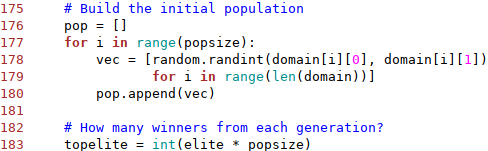
\includegraphics[width=0.7\textwidth]{pic/python_code.png}
            \caption{\label{fig:python_code}Python程序}
        \end{figure}

			与常见的动态类型语言一样,Python具有动态类型与垃圾回收机制,
      这两者保证了程序编写的方便性,使得人们能够更加专注与算法本身的实现而不被
      其他细节末枝干扰。并且
      Python具有庞大的标准库提供各式各样的封装函数,
      保证了程序的简洁性。相比于C++、Java或C\#之类的语言,Python语言编写的程序
      可读性高,代码简洁。 对于之后要实现的智能算法来说,Python语言可以带来快
      速开发、测试和修改等良好的特性。
		\subsection{团体旅游问题简介}
			为了能够具体说明航班选择问题的细节,本文所用示例是为来自不同地区又去往
      同一地点旅游的人安排购票方案,既选择不同的航班。在本例中有关乘客和他们来
      自何地的具体细节如表\ref{tab:family_info}所示,而他们的共同目的地则是LGA
      (位于纽约的机场)。从表格中来看,一共$6$人的团体旅游项目往返机票需要$12$张,
      我们需要做的是如何安排好这十二张机票的购买方案。
			\begin{table}[!htbp]
				\centering
				\caption{需要安排的成员信息}
				\label{tab:family_info}
				\begin{tabular}{c|cccccc}
					\toprule[1pt]
					姓名 & Seymour & Franny & Zooey & Walt & Buudy & Les \\
					\hline
					来自 & BOS     & DAL	  & CAK   & MIA  & ORD   & OMA \\
					\bottomrule[1pt]
				\end{tabular} 
			\end{table}
	并且由于是一次团体旅游活动,所以所有需要安排的成员都需要在同一天到达又要在
    同一天离开, 并且去机场时搭乘同样的交通工具。通过上面的了解我们知道,为了使旅行过程最
      优化我们需要尽可能的为每一位成员安排恰当的航班以达到出行的最优化配置,
      这就是航班选择的具体内容。
		\subsection{数据的获取与处理}
			我们从相关的航班网站中下载对应的航班数据并保存在文本文件中,之后算法
      会调用其中的数据来确定机票的各项信息。其中的数据包含以逗号分隔的不同航
      班的出发地点、目的地、起飞时间、到达时间、机票费用的信息。其中一项如下所示:
      \[LGA,OMA,6:20,12:22,942\]
	  它表达的含义是本次航班从$LGA$飞往$OMA$并且在早上$06:20$时起飞,并在
      下午$12:22$到达, 这张机票售价$942\$$, 在航班网站的订票界面显示如图\ref{fig:flight_example}。
			
        \begin{figure}[!h]
            \centering
            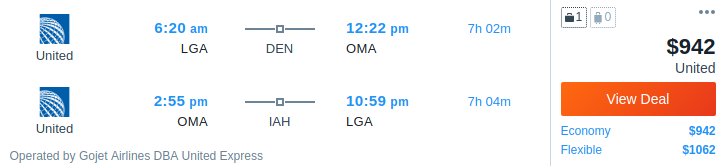
\includegraphics[width=0.7\textwidth]{pic/flight_example.png}
            \caption{\label{fig:flight_example}网站显示数据}
        \end{figure}
			
      为了能在Python程序中使用这些数据,我们将把这些数据加载为一个字典,
      字典是Python中的一种可变容器的模型,可存储任意类型对象。
      字典中包括键值与数据的对应。在此字典中
      以航班的起止点为键,详细信息为值。具体结构将如下所示:
			\begin{table}[!htbp]
				\centering
				\begin{tabular}{rl}
					$Dic\ = $ &$[$ \\
					&$\dots$ \\
					&$(LGA,OMA)=(6:20,12:22,942),$ \\
					&$\dots$\\
					&$]$
				\end{tabular} 
			\end{table}
			字典将在程序中被调用,查询时只需要知道键值就可以得到对应的航班信息,
            如$Dic[(LGA,OMA)]$将会给出$(6:20,12:22,942)$,这在算法实现中是非常方便的。
		\subsection{问题的程序实现}
			\label{sec:pdesc}
			为了简化航班选择在程序中的描述,我们把每个人所在地点一天中飞往纽约
            的航班按照时间顺序排列——$0$代表了一天中的第一次航班,$1$是第二次,
            以此类推。所以所有人所乘坐航班的选择可以描述为这样一个数组$[3,4,1,1,4,6]$。
            该数组的排列与表\ref{tab:family_info}相同,第一项的$3$表示Seymour
            将搭乘BOS的第三次航班飞往纽约。再加上返回时的航班选择最终结果将会是
            下面这样一个数组:
            \[S=[2,5,2,4,6,5,1,3,3,2,1,3]\]
			上述数组所对应航班列表如表\ref{tab:S_detail}所示。
			\begin{table}[!htbp]
				\centering
				\caption{具体安排的情况}
				\label{tab:S_detail}
				\begin{tabular}{ccccccc}
					\toprule[1pt]
					成员     & 出发地& 出发时间    &  价格  &  返回时间    &   价格 \\
					\midrule
					Seymour  & BOS &  9:45-11:50 & \$172 & 13:39-15:30 & \$ 74 \\
					Franny   & DAL & 13:54-18:02 & \$294 &  9:49-13:51 & \$229 \\
					Zooey    & CAK &  9:15-12:14 & \$247 & 12:01-13:41 & \$267 \\
					Walt     & MIA & 12:05-15:30 & \$330 & 15:23-18:49 & \$150 \\
					Buddy    & ORD & 15:58-18:40 & \$173 & 14:19-17:09 & \$190 \\
					Les      & OMA & 13:37-15:08 & \$250 &  8:04-10:59 & \$136 \\ 
					\bottomrule[1pt]
				\end{tabular} 
			\end{table}
			
			如果我们要对出行进行优化配置,那么最简单的优化方案既是让所有航班机
            票的价格最低即可,但是从表\ref{tab:S_detail}中可以看出,即使在同一
            天返回,时间的差别也是巨大的。即使忽略价格问题,由于团体旅行是成员
            一起往返于机场就会导致如果有成员的机票时间太早,而有些成员的时间又
            太晚造成时间上的浪费。为了解决这个问题,找到各个成本之间的平衡点,
            我们需要一种方法来为各个安排方案进行评估。
		\subsection{成本函数的确定}
            \label{sec:fitness_func}
			成本函数是优化算法的核心\upcite{王凌2001智能优化算法及其应用},在航
            班选择问题中成本函数的目标就是衡量一个选择方案的好坏程度。本文所讨
            论的优化算法的目的就是寻找到一组解使得成本函数的返回值最低。
			
			在复杂问题中确定成本函数,根据多个不同变量确认选择方案的优劣程度是
            比较困难的。因此在航班选择问题中,我们主要讨论如下几个影响因素:
			\begin{description}
				\item[价格因素] 机票所价格占据出行成本的大部分,因此在成本函数
                    中占据较大比重。
				\item[旅行时间] 每个人乘坐飞机所消耗的时间。
				\item[等待时间] 如果有成员的机票较早,那么其他成员将花费的等待成本。
				\item[出发成本] 如果出发时间较早,也会增加成员的出发成本,因为这
                    需要要求成员尽早起床。
				\item[车辆租用] 如果集体租用同一辆汽车,那么我们需要在同一天早
                    于租用时间返还车辆,否则将会多付一天租用费。
			\end{description}
			确定上述影响因素后,我们需要将所有因素结合为一个成本函数并且确定每
            个因素的重要性。根据不同因素的影响效果,成本函数将返回所有影响因素
            组合在一起的一个值。在航班选择问题中我们将在飞机上的时间成本设定为
            每分钟等价为一美元的成本,在机场等待的时间成本为每分钟等价0.5美元,
            这样我们就把时间成本与价格成本结合在了一起。
			
			结合机票的价格成本,飞行的时间成本,成员在机场等待的成本还有汽车租
            用的成本,最终我们可以得到成本函数的具体算法过程如下
            算法\ref{alg:evaluation}所示。
			\begin{algorithm}
                \begin{algorithmic}
					\caption{\label{alg:evaluation}成本函数}
					\Require $\text{航班选择序列S}$
					\Ensure $\text{序列S的出行成本C}$
					\Function {EvaluateCost}{$S$}
					\State $C \gets \Call {CostOfTicket}{S}$ \Comment 机票价格成本
					\State $C \gets C + \Call {CostOfTravel} {S}$ \Comment 飞行时间成本
					\State $C \gets C + \Call {CostOfWait} {S}$ \Comment 等待时间成本
					\State $C \gets C + \Call {CostOfEarly} {S}$ \Comment 出发时间成本
					\State $C \gets C + \Call {CostOfRent} {S}$ \Comment 汽车租用成本
					\State \Return{$C$}
					\EndFunction
                \end{algorithmic}
			\end{algorithm}
		
			其中在算法\ref{alg:evaluation}中的函数\Call {CostOfWait}{S}中,我们
            需要针对特殊情况做具体的处理。既我们允许任何需要等待两个小时或以上
            的人可以独自离开,具体算法实现如算法\ref{alg:CostOfWait}所示。
			\begin{algorithm}
				\begin{algorithmic}
					\caption{\label{alg:CostOfWait}等待时间成本}
					\Require $\text{航班选择序列S}$
					\Ensure $\text{序列S的等待时间成本C}$
					\Function {CostOfWait}{$S$}
					\State $S' \gets \Call {SortByLeftTime}{S[5:11]}$ \Comment 将返回时的序列按照时间排序
					\For {$i = 5 \to 11$} 
						\State $C \gets C + 0.5 \times i \times \Call {CostOfTime}{S'[i]}$ \Comment 时间成本
						\If {$(S'[i+1].LeftTime - S'[i].LeftTime) > 120$}\Comment 时间超过2小时
							\State $i \gets i + 1$ \Comment 跳过下一个成员
						\EndIf	
					\EndFor
					\State \Return{$C$}
					\EndFunction
				\end{algorithmic}
			\end{algorithm}
		
		成本函数确定后,
        我们需要找到方法使得成本函数的输出最小\upcite{陈冬芳2005全局最优化算法及其应用},
        既使得航班选择的最终成本最低。在航班选择问题中,出发与返回共有12个航班,
        每个航班又大约有10种可能。因此尝试每种可能并找出最优解是不太现实的,我们
        需要具体的优化算法来确定哪种方案才能使得成本函数取得最小值。之后本文将会使用Python
        语言建立不同的优化算法,并且针对每种算法做具体的测试与对比,并最终选择 
        效果最好的方案。
	\section{可行性分析}
		\subsection{技术可行性}
			Python语言致力于让程序变得简洁明了,
            让开发变得方便快捷\upcite{Oliphant2007Python},完全可以胜任航班选择
            优化算法的实现。从图\ref{fig:flight_example}中网站所给的
            航班数据中可以看出机票是成对出现的,也就是说每两个地点间都有往返机票,保证了不会出现无解的情况使算法出现问题。
		\subsection{操作可行性}
			算法程序由Python开发,而Python程序语言是一个跨平台语言。
            只要安装了对应的运行环境无论运行Windows、linux还是MacOS的电脑都可以无障碍使用,
            如图\ref{fig:linux_python}就是在linux系统上运行Python环境。
            \begin{figure}[!h]
                \centering
                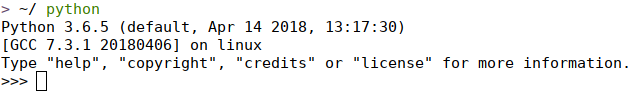
\includegraphics[width=0.7\textwidth]{pic/linux_python.png}
                \caption{\label{fig:linux_python}Python环境}
            \end{figure}
		\subsection{经济可行性}
			开发算法所用到的程序语言开发工具完全免费,并可以在官网下载。
            机票订购网站的数据也可以自由访问,而无需付费,完全具有经济可行性。
	\section{问题求解}
	\label{sec:solve}
		\subsection{本章结构}
			为了选出最优算法,在本章中将会实现四种不同优化算法,通过运行不同优
            化算法处理已有的航班数据
            得到结果。然后成本函数对比各个算法所得出的结果的优劣,选出效果最好的优化算法,
            其具体流程如图\ref{fig:flow}所示。
			\begin{figure}[!h]
				\centering
				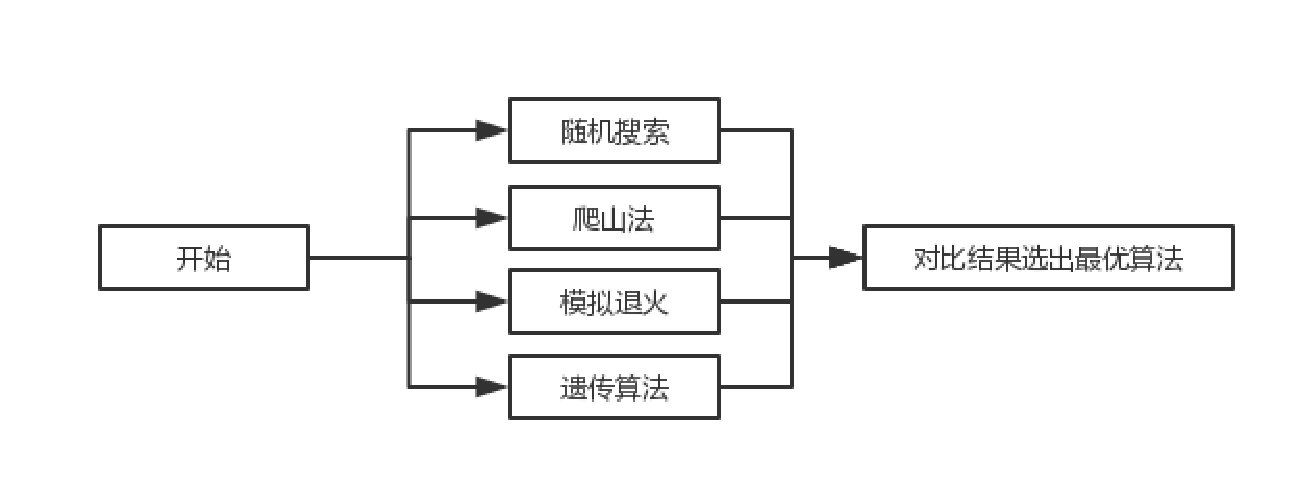
\includegraphics[width=0.8\textwidth]{pic/flow.pdf}
				\caption{\label{fig:flow}本章主要流程}
			\end{figure}
		\subsection{随机搜索}
		\label{sec:random}
			随机搜索的本质是随机猜测可能的安排方案并且通过与之前方案的对比,
            通过成本函数找到可行的解\upcite{贺红2002随机算法的一般性原理}。
			
			加入随机搜索算法是为了与其后要讨论的其他优化算法做对比,以衡量算法
            的优劣,并介绍一般优化算法的调用过程与基本结构。随机搜索算法的结构
            如算法\ref{alg:randomsearch}所示。
			\begin{algorithm}
				\begin{algorithmic}
					\caption{\label{alg:randomsearch}随机搜索}
					\Require $\text{可选的航班号序列D}$
					\Ensure $\text{航班序列S}$
					\Function {RandomSearch}{$D$}
					\State $Best \gets 100000$ \Comment 成本初始化为一个大数
					\For {$i = 0 \to 1000$}  \Comment 随机搜索1000次
						\State $S' \gets [ \Call{Random}{0,D[i]}\ \textbf{for}\ i\ \textbf{in}\ \Call{Len}{D}]$ \Comment 随机生成一个航班序列
						\If {$\Call{EvaluateCost}{S} < Best$} \Comment 如果比上一最好的成本更低
							\State $Best \gets \Call{EvaluateCost}{S}$ \Comment 设置当前为最优
							\State $S \gets S'$ \Comment 更新最优航班序列
						\EndIf
					\EndFor
					\State \Return{$S$}
					\EndFunction
				\end{algorithmic}
			\end{algorithm}
		
			作为一个对比基准,随机搜索的结果如表\ref{tab:random}所示,其中的序
            列既为\ref{sec:pdesc}\ 中的航班序列。
			\begin{table}[!htbp]
				\centering
				\caption{随机搜索算法得出的结果}
				\label{tab:random}
				\begin{tabular}{ccccccc}
					\toprule[1pt]
					成员     & 出发地& 出发时间    &  价格  &  返回时间    &   价格 \\
					\midrule
					Seymour   &    BOS & 18:34-19:36 & \$136  & 8:23-10:28 & \$149 \\
					Franny    &   DAL  & 7:53-11:37 & \$433 & 19:57-23:15 & \$512 \\
					Zooey     &  CAK & 20:30-23:11 & \$114 & 18:17-21:04 & \$259 \\
					Walt      & MIA & 18:23-21:35 & \$134 & 12:37-15:05 & \$170 \\ 
					Buddy     &  ORD & 12:44-14:17 & \$134 & 14:19-17:09 & \$190 \\
					Les       & OMA & 13:37-15:08 & \$250 & 16:35-18:56 & \$144 \\
					\midrule
					序列    & \multicolumn{5}{c}{[8, 1, 9, 8, 4, 5, 7, 1, 8, 6, 1, 6]}\\
					成本    & \multicolumn{5}{c}{6234} \\
					\bottomrule[1pt]
				\end{tabular} 
			\end{table}
		\subsection{爬山算法寻找最优解}
			从\ref{sec:random}可以看出随机搜索的效率是十分地下的。在随机搜索中
            我们只能盲目的寻找下一个可能的选择方案而没有利用我们已经找到的较好
            的解。在航班选择问题中一个较好的选择方案的解很可能与其他较好方案的
            解接近。为了能够利用好已被发现的较好的选择方案而发现更优的方案,我
            们使用一个能搜索临近更优解的算法。
			\subsubsection{算法的描述}
			爬山算法从一个已有的选择方案开始,在这个选择方案临近的解集中寻找更
            好的解决方案。这类似于爬山从山坡上向下走,如图\ref{fig:around_search}所示。
			\begin{figure}[!h]
				\centering
				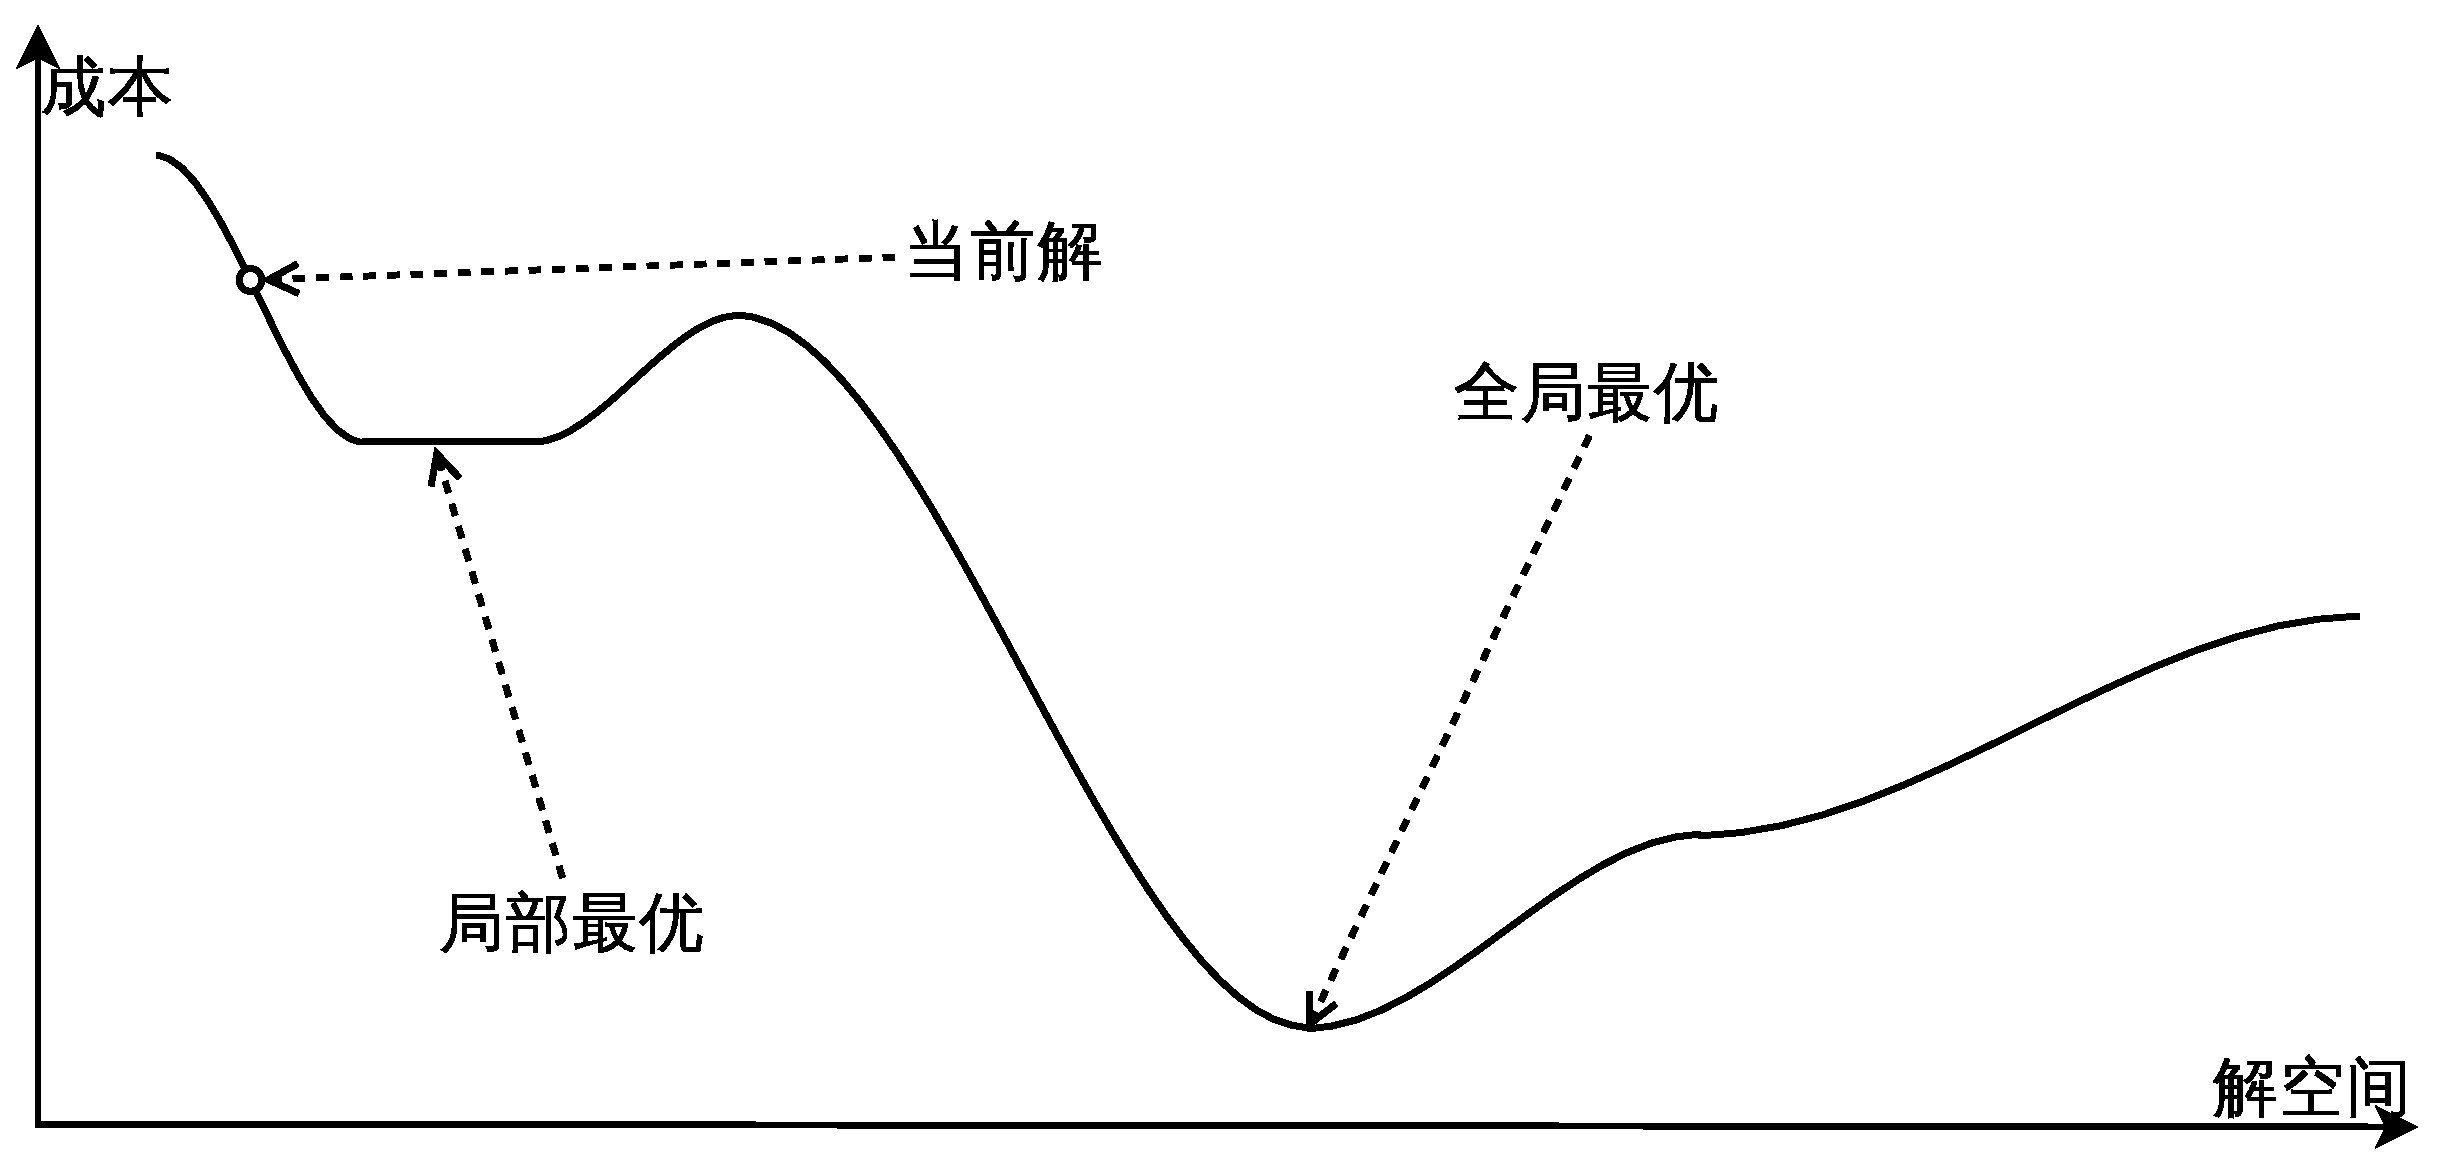
\includegraphics[width=0.7\textwidth]{pic/around_search.eps}
				\caption{\label{fig:around_search}爬山法}
			\end{figure}
			在图中当前解处算法将根据当前解左右的成本取值找到一个更优解,也就是
            当前解的右边。最终根据算法当前解会顺着斜坡一直走下去,
            直到没有更优解\upcite{Huhn2007Interior}。
			
			在航班选择问题中使用爬山算法解决问题的关键是,先随机生成一个航班选
            择方案,然后再寻找与之相临的方案。在相邻的方案中寻找更优方案。
			
			在本例中我们将与当前方案相比可以让某人乘坐的航班稍早或稍晚的方案作
            为相邻解。我们对每个搜索到的方案进行成本计算,并且安排在相邻解集中
            的最优解作为下一次的初始解,具体算法如算法\ref{alg:around_search}所示。
            \begin{algorithm}
				\begin{algorithmic}
					\caption{\label{alg:around_search}爬山算法}
					\Require $\text{可选的航班号序列D}$
					\Ensure $\text{航班序列S}$
					\Function {HillClimbSearch}{$D$}
					\State $S \gets [ \Call{Random}{0,D[i]}\ \textbf{for}\ i\ \textbf{in}\ \Call{Len}{D}]$ \Comment 随机生成一个航班序列
					\While {$True$}
						\State $Neighbors \gets [\ ]$ \Comment 相邻解的列表
						\For {$i = 0 \to \Call{Len}{D}$} \Comment 生成临近解集
							\If {$S[i] > D[i][0]$} \Comment 如果某人航班号大于起始航班号
								\State $S[i] \gets S[i] - 1$ \Comment 选择到更小的航班号
								\State $Neighbors.Append(S)$ \Comment 加入到相邻解集中
							\Else \Comment 是起始航班号
								\State $S[i] \gets S[i] + 1$ \Comment 选择到更大的航班号
								\State $Neighbors.Append(S)$ \Comment 加入到相邻解集中
							\EndIf
						\EndFor
						\State $Best \gets \Call{EvaluateCost}{S}$ \Comment 保存上次最优解
						\For {$S'\ \textbf{in}\ Neighbors$}
							\If {$\Call{EvaluateCost}{S'} < \Call{EvaluateCost}{S}$} \Comment S'为更优解
								\State $S \gets S'$ \Comment 把更优解赋值给S
							\EndIf
						\EndFor
						\If {$\Call{EvaluateCost}{S} = Best$} \Comment 如果没有更好的解
							\State $Break$ \Comment 跳出循环
						\EndIf
					\EndWhile
					\State \Return{$S$}
					\EndFunction
				\end{algorithmic}
            \end{algorithm}

			最终爬山法所获得的结果如表\ref{tab:hillclimb}所示,可以看出使用了更
            加可行的算法后,爬山法与随机搜索相比有了很大进步。

			\begin{table}[!htbp]
			\centering
			\caption{爬山算法得出的结果}
			\label{tab:hillclimb}
			\begin{tabular}{ccccccc}
				\toprule[1pt]
				成员     & 出发地& 出发时间    &  价格  &  返回时间    &   价格 \\
				\midrule
				Seymour   &    BOS & 18:34-19:36 & \$136 & 10:33-12:03 & \$ 74 \\
				Franny    &   DAL & 10:30-14:57 & \$290 & 18:44-22:42 & \$351 \\
				Zooey     &  CAK & 18:35-20:28 & \$204 & 10:32-13:16 & \$139 \\
				Walt      & MIA & 11:28-14:40 & \$248 & 18:07-21:30 & \$355 \\
				Buddy     &  ORD & 18:48-21:45 & \$246 & 14:19-17:09 & \$190 \\
				Les       & OMA & 13:37-15:08 & \$250 & 11:07-13:24 & \$171 \\	
				\midrule
				序列    & \multicolumn{5}{c}{[8, 3, 8, 3, 8, 5, 3, 4, 8, 3, 4, 6]} \\
				成本    & \multicolumn{5}{c}{4079} \\
				\bottomrule[1pt]
			\end{tabular} 
			\end{table}
			

			\subsubsection{局部最优解}
			爬山算法的效果一般比随机搜索的效果要好,
            但爬山算法有个重要缺陷\upcite{Xiao2004A}。
            从图\ref{fig:local_best}可以看出,如果爬山算法如果找不到比当前最
            优解更好的解,它就会陷入局部的最优解而无法跳出。

            一般来说对于在\ref{sec:fitness_func}中建立的适应度函数,我们将其
            记为$f(s)$,其中$s$代表了不同的方案,$S$则是所有方案的集合。
            那么对于$f(s)$的全局最优解与局部最优解为
            \begin{align*}
                f(s_0) &= min\{f(s)\} \qquad s_0,s \in S \\
                f(d_0) &= min\{f(d)\} \qquad d_0,d \in D \quad D \subset S
            \end{align*}

            在图\ref{fig:local_best}中如果爬山算法的初始解生成在虚线左边,
            如$A$点和$B$点,那么根据算法中的永远只找更好的解的规则,对于$A$点,
            解会逐渐向右前进。对于$B$点则会向左前进,最终
            在爬山算法的运行逻辑下最终都会陷入$C$点而不能到达全局最优。
            
			\begin{figure}[!htbp]
				\centering
				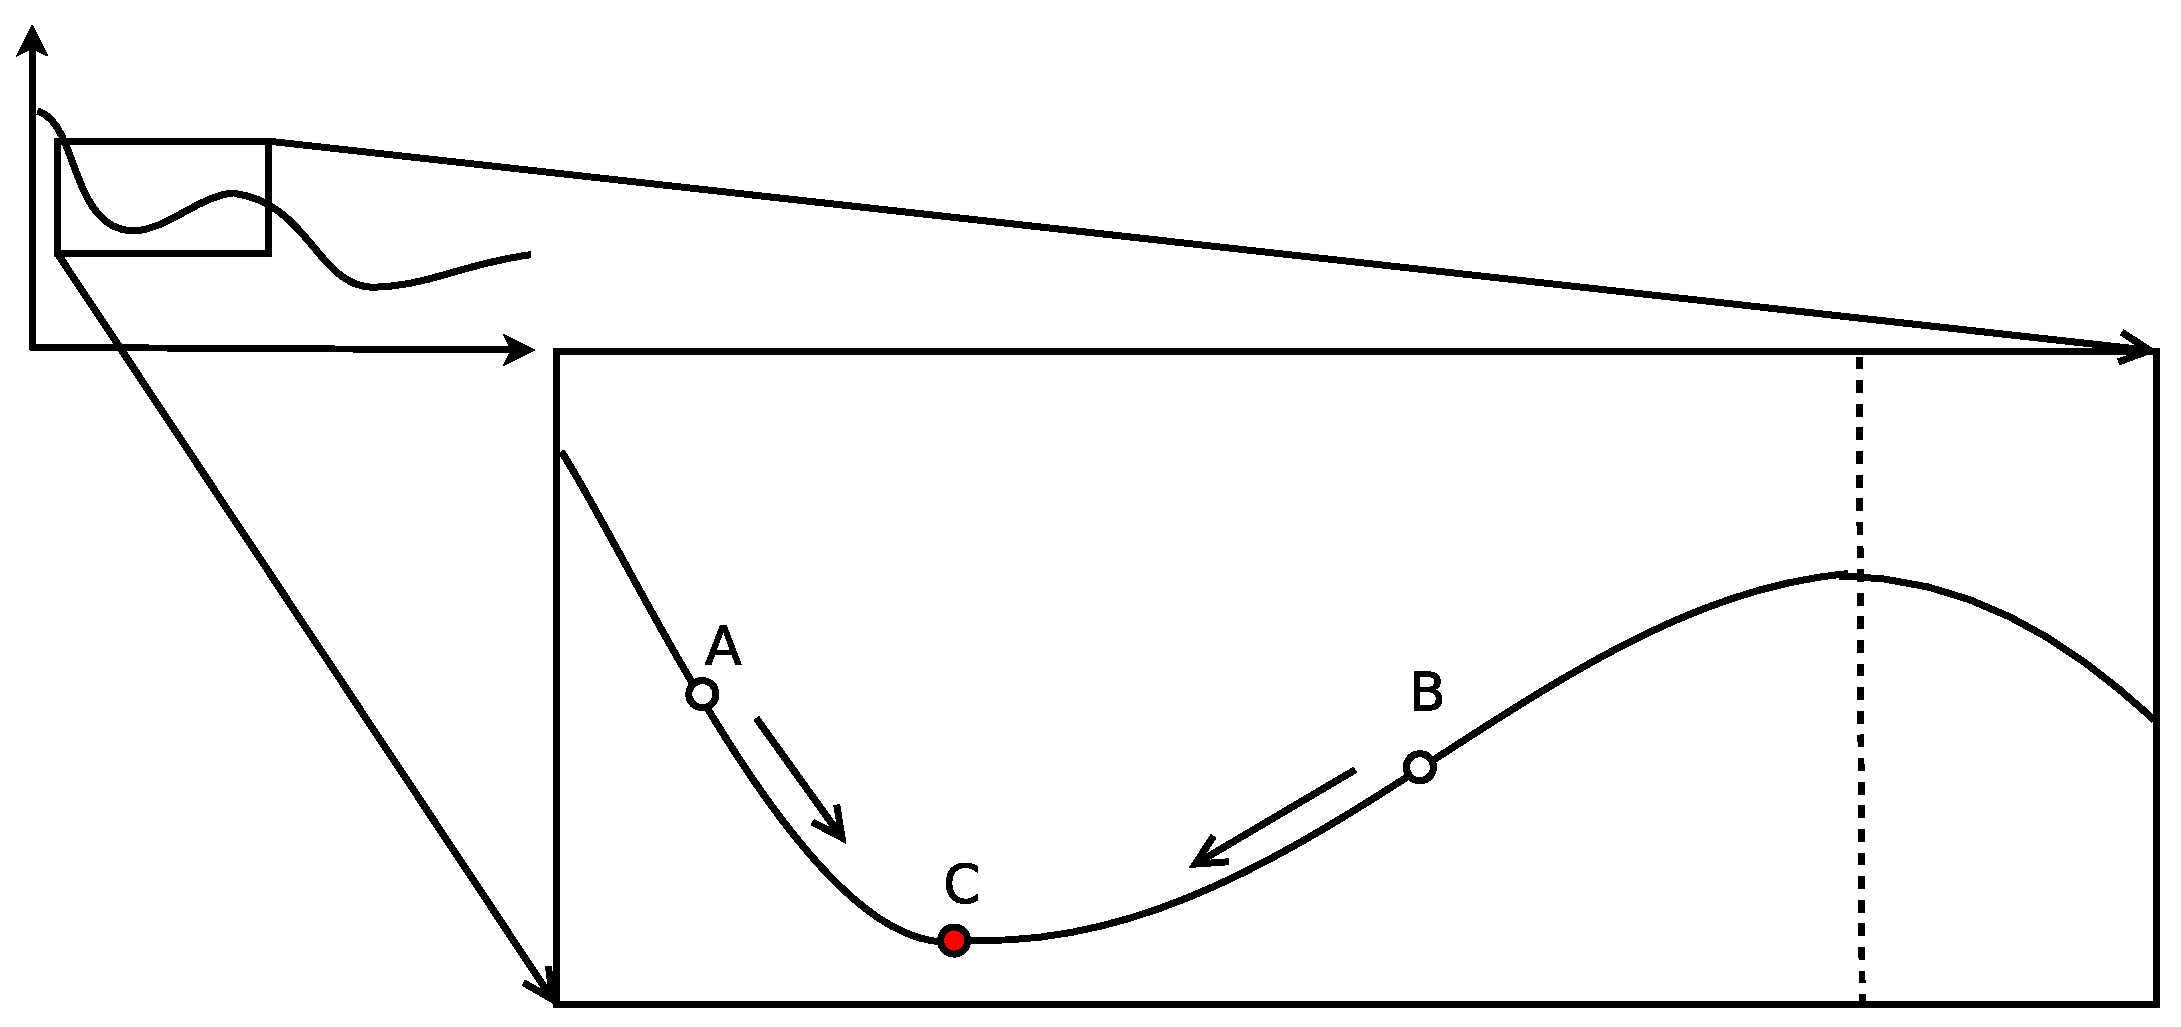
\includegraphics[width=0.7\textwidth]{pic/local_best.eps}
				\caption{\label{fig:local_best}局部最优解}
			\end{figure}

			而局部的最优解不一定是全局的最优解,为了解决爬山算法容易陷入局部最
            优的问题。我们需要更加智能,能够跳出局部最优解找到全局最优解的优化算法。
		\subsection{模拟退火算法}
			模拟退火算法是用来给定近似全局最优解的启发式算法之一,它可以解决上述
            局部最优解的问题。
			这个名称的灵感来自于冶金学上的退火,一种涉及材料加热和控制冷却以增
            加晶体尺寸并减少其缺陷的技术。
			
			\subsubsection{模型的建立}
			模拟退火同样从一个随机解出发,在每次迭代过程中,算法会随机选择解中
            的某个元素进行改变。如果得到的结果更好,即成本函数更低,这个最优解
            将会成为下一次迭代的开始\upcite{王雪梅1997模拟退火算法与遗传算法的结合}。
			与上述爬山法不同的是,即使某个解可能看起来更差,模拟退火算法仍有可
            能将它当作下一次迭代的开始。这是因为算法引入了温度参数$T$来控制接受
            较差解的程度。
			
			
			\begin{figure}[!h]
				\centering
				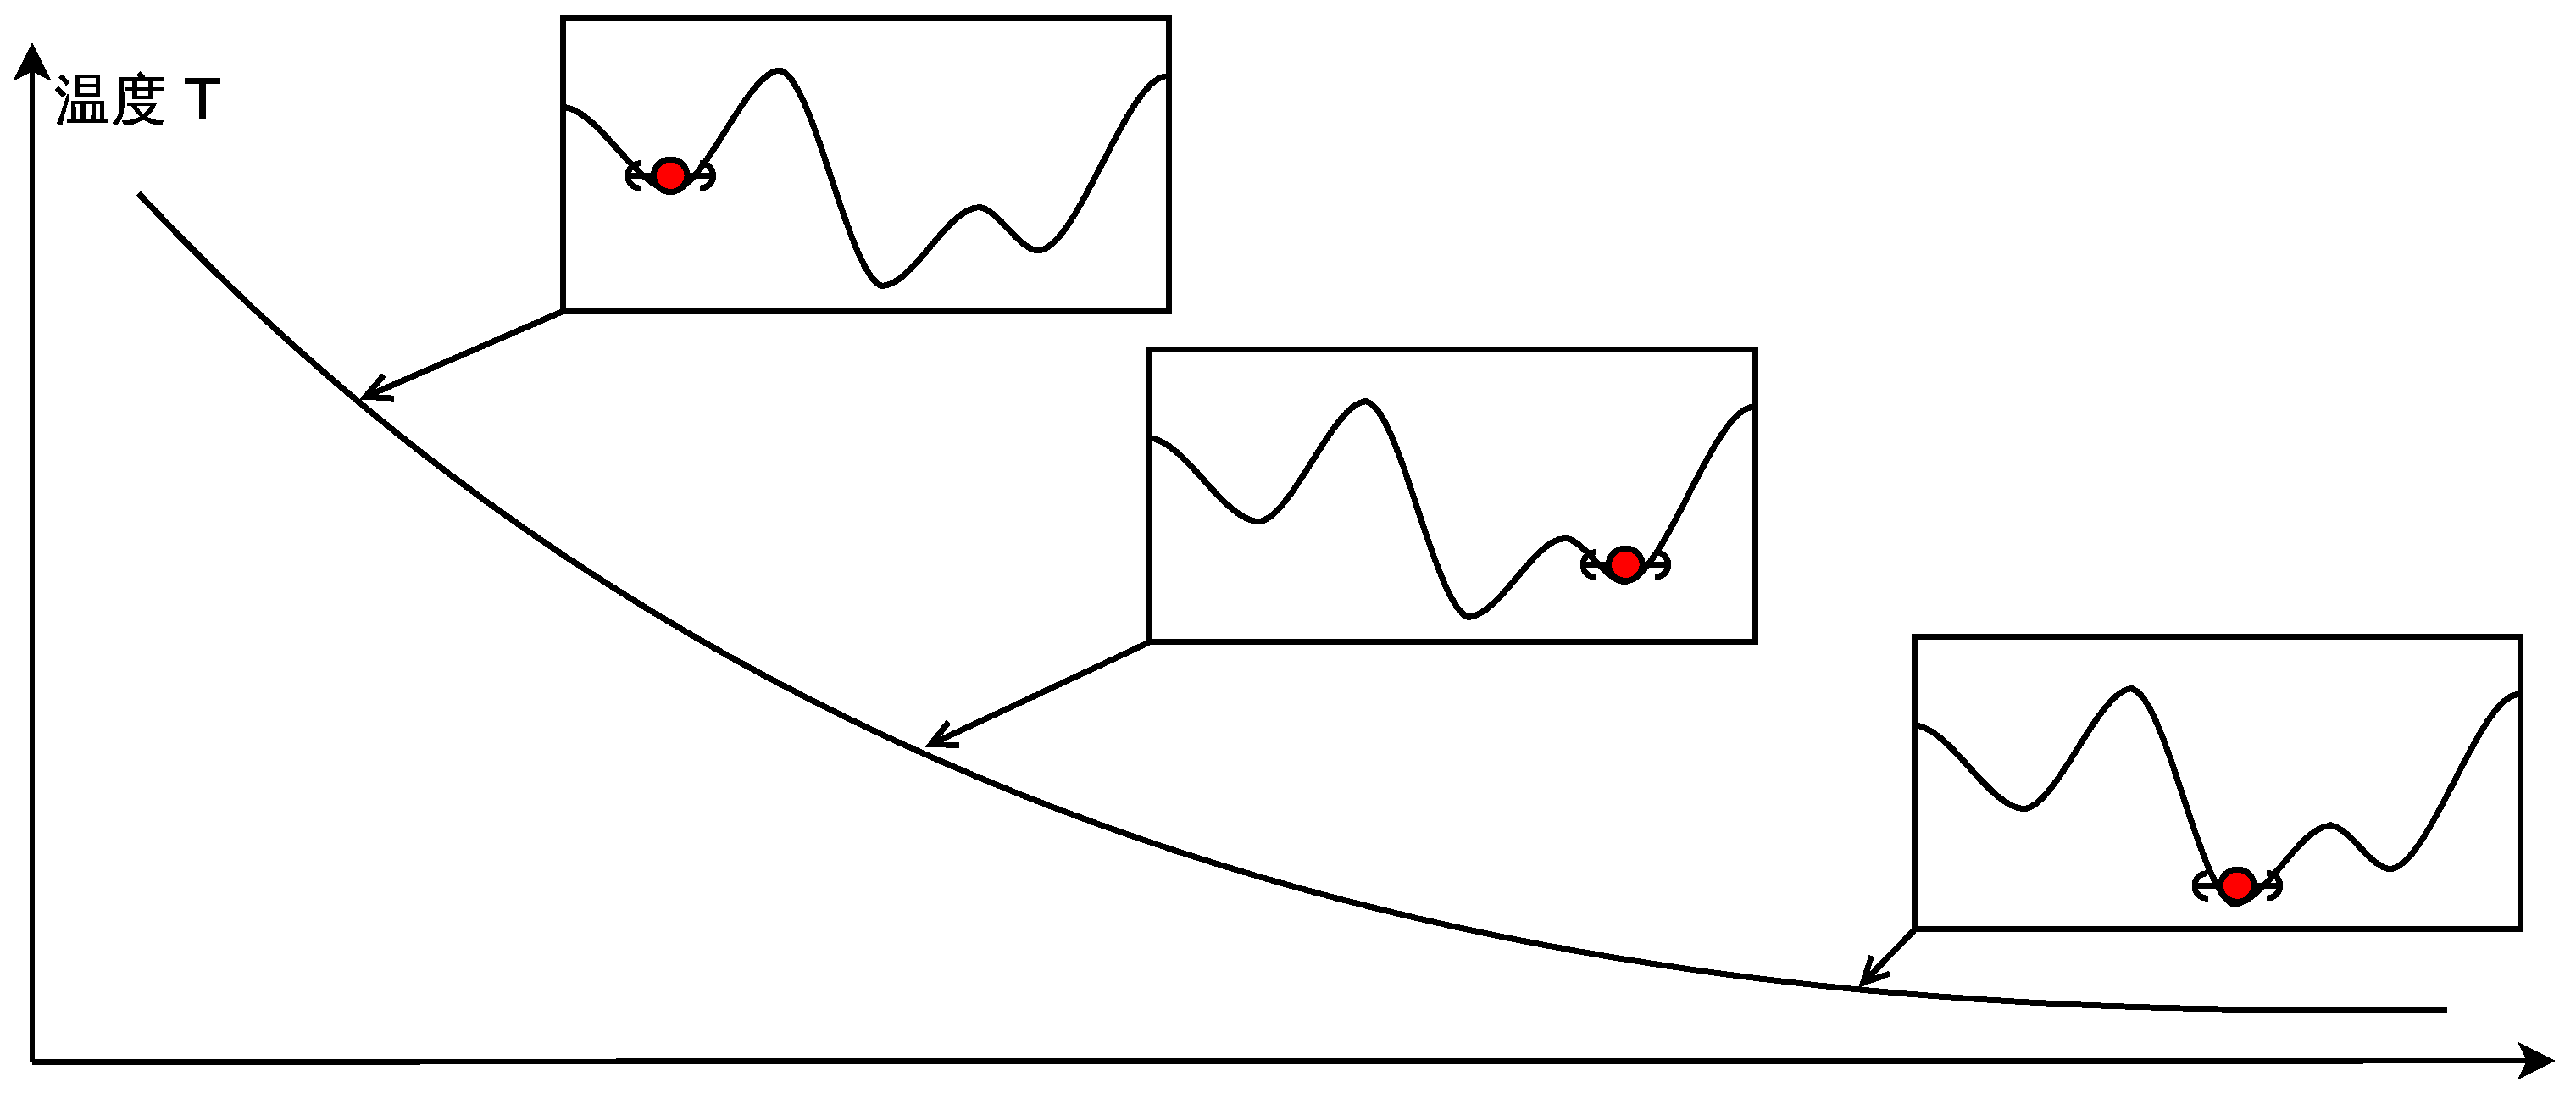
\includegraphics[width=0.7\textwidth]{pic/annle.eps}
				\caption{\label{fig:annle}模拟退火算法}
			\end{figure}
			算法的迭代过程如图\ref{fig:annle}所示,随着温度$T$的降低,算法也越
            来越接近全局最优解。
			在模拟退火算法最开始的阶段算法会更容易接受那些比较差的解,随着
            温度$T$的降低算法将会变得越来越不能接受更差的解,直到算法的最后阶段
            ,模拟退火将要完成时,
            算法只会接受更优的解\upcite{高尚2002模拟退火算法中的退火策略研究}。
			在算法运行过程中,更高成本的解能被接受的程度与温度的关系由
            公式\ref{eq:p_func}所示\upcite{Kirkpatrick1987Optimization},
            其中$h$代表了更高成本解的成本,$l$代表了原本解的成本。
			\begin{equation}
			p=e^{-\frac{h-l}{T}}
			\label{eq:p_func}
			\end{equation}
			
			从公式\ref{eq:p_func}可以看出,在最开始时模拟退火算法的温度非常高,
            因此$p$的值将会非常接近$1$。即代表此时系统几乎完全接受成本最高的解,
            随着温度$T$的下降,$p$的值将会越来越接近$0$。
			综上所述,具体程序如算法\ref{alg:annealing_search}所示。
			\begin{algorithm}
				\begin{algorithmic}
					\caption{\label{alg:annealing_search}模拟退火算法}
					\Require $\text{可选的航班号序列D,初始温度T,降温比率C}$
					\Ensure $\text{航班序列S}$
					\Function {AnnealingSearch}{$D,T=10000,C=0.95$}
					\State $S \gets [ \Call{Random}{0,D[i]}\ \textbf{for}\ i\ \textbf{in}\ \Call{Len}{D}]$ \Comment 随机生成一个航班序列
					\While {$T>0.1$} \Comment 在温度降低之前一直循环
						\State $l \gets \Call{Len}{S}$ \Comment 获得序列的长度
						\State $i \gets \Call{Random}{0,l}$ \Comment 随机选择一项进行改变
						\State $s \gets \Call{Random}{-1,1}$ \Comment 随机选择改变方向
						\State $S' \gets S$ \Comment 生成下一解
						\State $S'[i] \gets S'[i] + s$ \Comment 应用更改,随机变化
						\State $ea \gets \Call{EvaluateCost}{S}$ \Comment 先前解的成本
						\State $eb \gets \Call{EvaluateCost}{S'}$ \Comment 下一解的成本
						\If {$ea < eb\ \textbf{or}\ \Call{Random}{0,1} < e^{-(eb-ea)/T}$} \Comment 模拟退火概率
							\State $S \gets S'$ \Comment 赋值给下一解
						\EndIf
						\State $T \gets T \times C$ \Comment 降温
					\EndWhile
					\State \Return{$S$}
					\EndFunction
				\end{algorithmic}
			\end{algorithm}
		
			最终通过模拟退火算法得到的结果如表\ref{tab:annealing}所示,可以看到
            模拟退火的结果相比随机搜索与爬山算法都要优秀。同时,对比三个算法的
            时间复杂度可以发现,退火算法的执行时间明显减少。
			\begin{table}[!htbp]
				\centering
				\caption{模拟退火算法得出的结果}
				\label{tab:annealing}
				\begin{tabular}{ccccccc}
					\toprule[1pt]
					成员     & 出发地& 出发时间    &  价格  &  返回时间    &   价格 \\
					\midrule
					Seymour  &      BOS & 17:11-18:30 & \$108 &  8:23-10:28 & \$149 \\
					Franny   &   DAL  & 7:53-11:37 & \$433  & 6:09- 9:49 & \$414 \\
					Zooey    &   CAK  & 6:08- 8:06 & \$224 & 13:37-15:33 & \$142 \\
					Walt     &  MIA & 14:01-17:24 & \$338 & 15:23-18:49 & \$150 \\
					Buddy    &   ORD & 15:58-18:40 & \$173 & 10:33-13:11 & \$132 \\
					Les      & OMA  & 11:08-13:07 & \$175 & 15:07-17:21 & \$129 \\
					\midrule
					序列    & \multicolumn{5}{c}{[7, 1, 0, 5, 6, 3, 6, 1, 6, 1, 6, 1]} \\
					成本    & \multicolumn{5}{c}{3679} \\
					\bottomrule[1pt]
				\end{tabular} 
			\end{table}
		\subsection{遗传算法}
			遗传算法是模仿生物进化过程的一种算法,它以自然选择和遗传学中的复制、
            变异和交叉等自然规律为理论依据。利用遗传算法求解航班选择问题,首先
            需要算法随机生成初始种群,即一组初始的可行解,再重复对种群进行选择、交
			叉、变异等遗传操作直到种群成熟\upcite{赵静2008数学建模与数学实验}。
            然后根据成本函数对整个种群的适应度即成本进行排序,成本越低,适应度越高。
			
			
			\subsubsection{变异与交叉算子}
			\label{sec:ag_cal}
			为了能更好的在航班选择问题中使用遗传算法,我们将个体的适应度,也就是
            成本加入个体的基因中,构成的种群个体结构如图\ref{fig:life}所示。
			\begin{figure}[htbp]
				\centering
				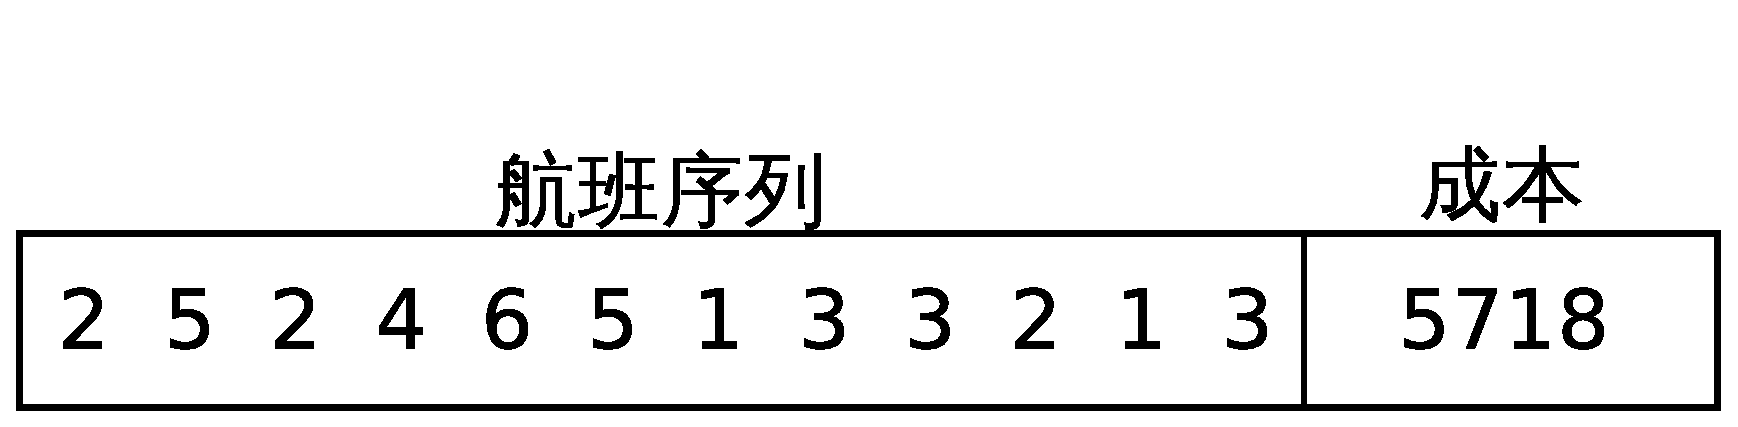
\includegraphics[width=0.6\textwidth]{pic/life_struct.eps}
				\caption{种群中的个体}
				\label{fig:life}
			\end{figure}
		
			种群中被选出的一组新的最优解是由之前种群按照适应度排序后稍做修改得
            来的\upcite{张铃2000遗传算法机理的研究},其中突变算子是指让种
			群中某个个体的某些基因突变的算子,其 在种群迭代中其过程
            如图\ref{fig:muate}所示,变异不一定是好的,通常情况下变异会使基因的
            适应度减小,即成本增大,但变异给算法提供了一种搜索全局最优解的
            可能\upcite{Goldberg1989Genetic}。
			\begin{figure}[!htbp]
				\centering
				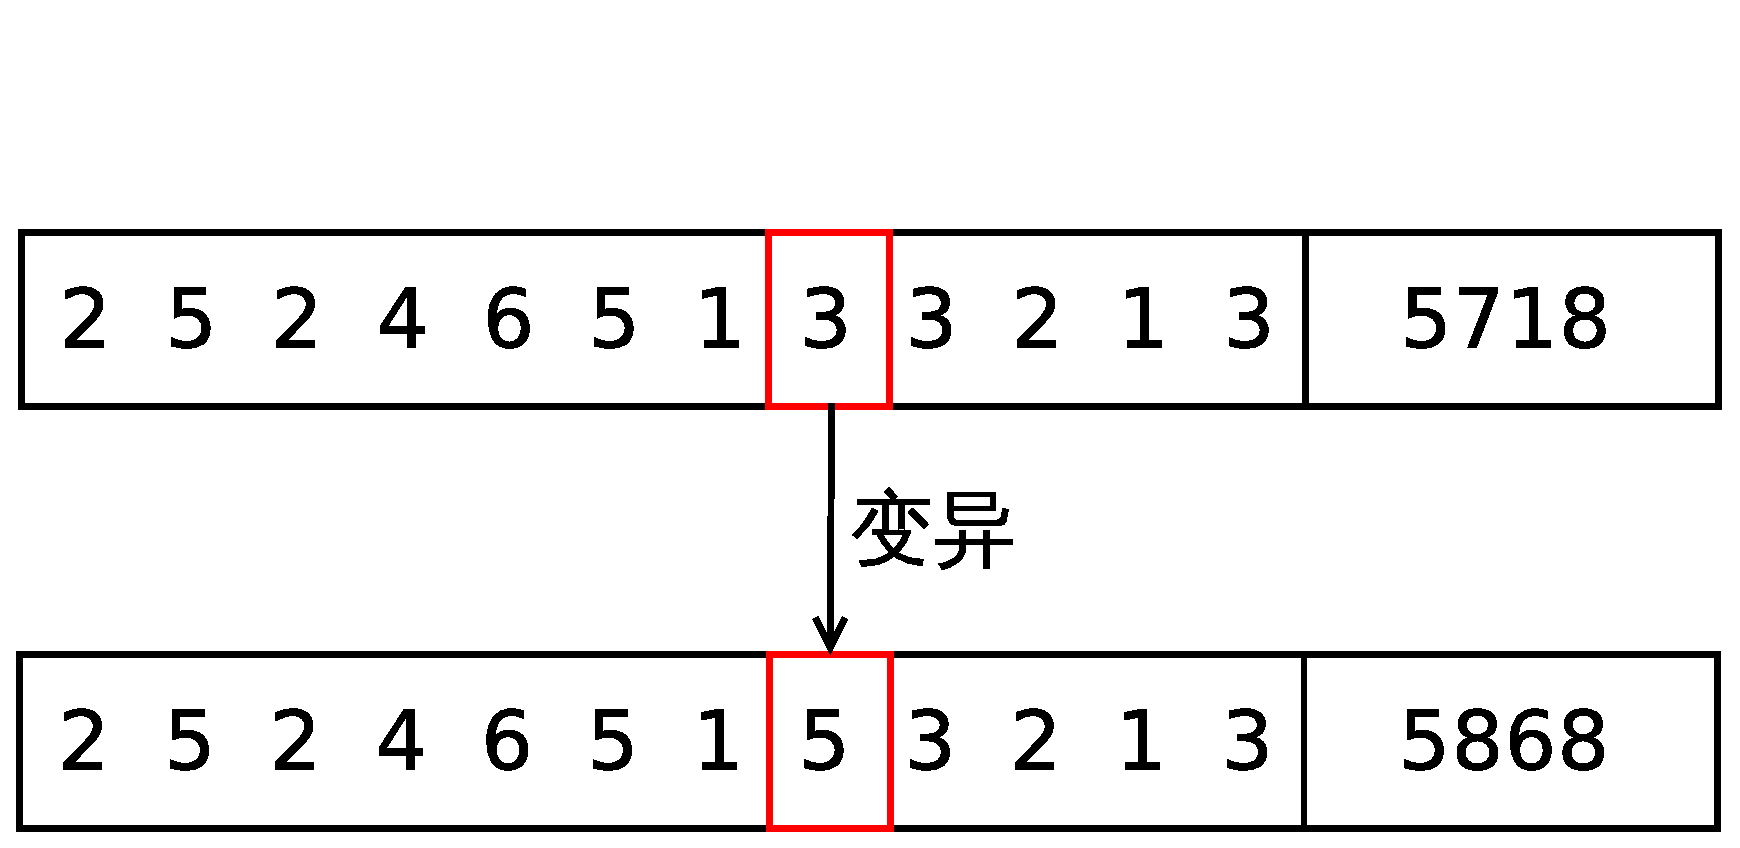
\includegraphics[width=0.6\textwidth]{pic/life_muate.eps}
				\caption{突变算子}
				\label{fig:muate}
			\end{figure}
			
			同样的对于算法中的交叉算子\upcite{胡中功2008群智能算法的研究进展},
            它是使有效基因遗传下去的主要算子,在交叉过程中算法随机选取一个交叉
            点并在交叉点随机选取一个不定长度的序列。于此同时在另一个个体中也选
            取同样长度的一条序列,双方个体交换这个序列即为交叉过程,
            如图\ref{fig:cross}所示。
			\begin{figure}[!htbp]
				\centering
				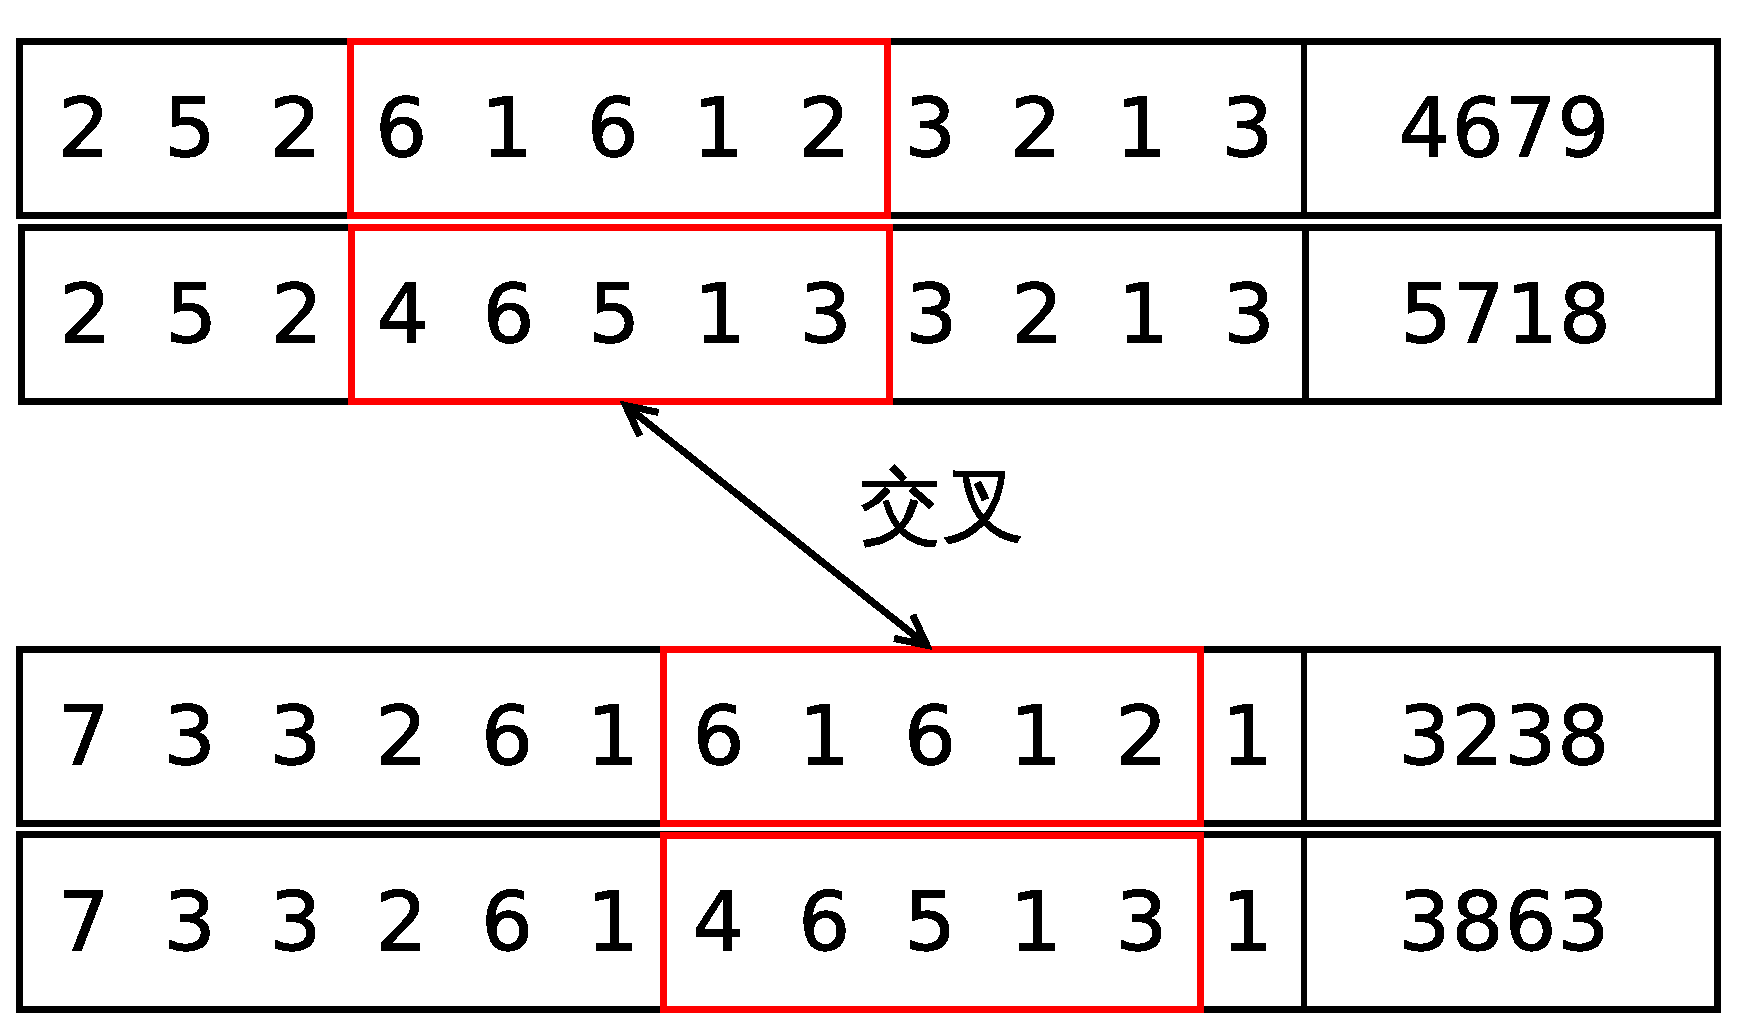
\includegraphics[width=0.6\textwidth]{pic/life_cross.eps}
				\caption{交叉算子}
				\label{fig:cross}
			\end{figure}
		
			上述两种算子是遗传算法中常用的用来寻找全局最优解,或者跳出局部最优
            解的搜索方案\upcite{苗夺谦1999知识约简的一种启发式算法}。在航班选择
            问题中使用变异和交叉算子将会使算法能够更好地搜索到最终的优化方案。
            从图\ref{fig:cross}来看当一个适应度较低的个体与适应度较高的个体交叉时,
            适应度较高个体的优秀基因成功降低了原个体的成本,既提高了个体的适应度。
			\subsubsection{算法的执行过程}
			正如\ref{sec:ag_cal}中描述的,遗传算法通过变异与交叉算法从已有的种群
            中构造一个新的种群,之后又以新的种群开始构造下一个种群。经过足够长的
            时间的迭代,遗传算法所得到的解将会越来越优越,
            具体实现如算法\ref{alg:ga_search}所示。
			\begin{algorithm}
				\begin{algorithmic}
					\caption{\label{alg:ga_search}遗传算法}
					\Require $\text{可选的航班号序列D,种群数量N,变异比率M,交叉比率E}$
					\Ensure $\text{航班序列S}$
					\Function {GeneticSearch}{$D,N=500,M=0.2,E=0.2$}
					\State $Pop \gets [\ ]$
					\For {$i\ \textbf{in}\ \Call{Range}{N}$} \Comment 生成初始种群
						\State $S \gets [ \Call{Random}{0,D[i]}\ \textbf{for}\ i\ \textbf{in}\ \Call{Len}{D}]$ \Comment 随机生成一个航班序列
						\State $Pop.Append([S,\Call{EvaluateCost}{S}])$ \Comment 加入种群
					\EndFor
					
					\For {$i\ \textbf{in}\ \Call{Range}{100}$} \Comment 循环100代
						\State $Elite = \Call{Sort}{Pop,Pop[][-1]}[0:0.2 \times N]$ \Comment 选出适应度最好的20\%
						\While {$\Call{Len}{Pop} < N$} \Comment 当种群未满时
							\If {$\Call{Random}{0,1} < M$}
								\State $Pop.Append(\Call{Muate}{Elite})$ \Comment 添加变异个体
							\EndIf
							\If {$\Call{Random}{0,1} < E$}
							\State $Pop.Append(\Call{Cross}{Elite})$ \Comment 添加交叉个体
							\EndIf
						\EndWhile
					\EndFor
					\State $S \gets Elite[0][0:-1]$ \Comment 返回种群中最好的个体
					\State \Return{$S$}
					\EndFunction
				\end{algorithmic}
			\end{algorithm}
		
			从表\ref{tab:ga}来看,最终得到的结果相比于上面提到过的所有算法都要好,
            对比模拟退火算法的结果可以看出即使两种算法都能跳出局部最优解,但遗
            传算法的全局最优解搜索能力要好于模拟退火算法。
			\begin{table}[!htbp]
			\centering
			\caption{遗传算法得出的结果}
			\label{tab:ga}
			\begin{tabular}{ccccccc}
				\toprule[1pt]
				成员     & 出发地& 出发时间    &  价格  &  返回时间    &   价格 \\
				\midrule
				Seymour  &     BOS & 12:34-15:02 & \$109 &  8:23-10:28 & \$149 \\
				Franny   &    DAL &  7:53-11:37 & \$433 & 10:51-14:16 & \$256 \\
				Zooey    &   CAK & 10:53-13:36 & \$189 &  9:58-12:56 & \$249 \\
				Walt     &  MIA  & 9:15-12:29 & \$225 & 12:37-15:05 & \$170 \\
				Buddy    &   ORD & 12:44-14:17 & \$134 &  7:50-10:08 & \$164 \\
				Les      & OMA  & 7:39-10:24 & \$219 & 11:07-13:24 & \$171 \\
				\midrule
				序列    & \multicolumn{5}{c}{[4, 1, 3, 2, 4, 1, 3, 1, 4, 1, 4, 1]} \\
				成本    & \multicolumn{5}{c}{2404} \\
				\bottomrule[1pt]
			\end{tabular} 
			\end{table}
		
	\newpage
	
	\section{总结与展望}
	\label{sec:conclude}
		\subsection{结果分析}
			根据我们在第\ref{sec:solve}\ 章中算法的使用与求解,可以看出随机搜
            索作为对比的基准首先介绍,但随机搜索效果太差,基本上很难给出令人满
            意的结果;作为对随机搜索的优化爬山法提供了一个更合理的
            思路\upcite{Thomas2013算法导论},即根据当前解来找到下一个解,只接
            受更优解,但爬山法的方式决定了它的固有缺陷,即难以跳出局部最优解。
			
			而为了解决爬山法容易陷入局部最优解而无法跳出的问题我们引入了模拟退
            火算法,它由物理模型引入在算法的初期可以有效的跳出局部最优解,找到
            全局最优解;作为模拟退火的对比,遗传算法通过模拟生物群落进化的方式
            交换优秀基因,具有更高的全局搜索性,能够更好的找到选择方案。
			
			
			\begin{table}[!htbp]
				\centering
				\caption{四种算法对比结果}
				\label{tab:cmp}
				\begin{tabular}{cc}
					\toprule[1pt]
					\makebox[0.3\textwidth]{算法} & \makebox[0.3\textwidth]{方案成本} \\
					\midrule
					随机搜索 		& 6234 \\
					爬山法			 &  4079 \\
					模拟退火算法	   & 3679 \\
					遗传算法		&  2404 \\
					\bottomrule[1pt]
				\end{tabular} 
			\end{table}
		
			综上所述,对比四种优化算法实验中得到结果总结如表\ref{tab:cmp}所示,
            从中可以看出遗传算法所得到的方案成本最低,即遗传算法最适合于航班选择问题。
		\subsection{解决问题意义}
			在生活节奏不断加快的现代社会,无论任何问题如何快速而又正确地找到解决
            方案是本文所要讨论的。航班选择是其中具有代表性的一个问题,通过文中优
            化算法的使用,我们最终优化了出行成本,相比于随机作出的决定优化算法所
            给出的方案成本降低了159\%,这大大降低了出行所需的成本节约了时间与金
            钱,提高了效率。
		\subsection{进一步工作与展望}
			为了能让更多人了解优化算法的作用,降低人们的生活成本,我们接下来的工
            作可以将优化算法与航空公司的订单网站结合起来,为出行的人们提供在线的
            实时的服务。当人们在网站上预订机票时,后台系统将会自动给出优化结果,
            给出建议。实现网络上的订单优化,这将节约大量社会成本。
	\newpage

	\bibliographystyle{gbt7714}	
	\bibliography{mybib}
	\newpage
	\section{致谢}
		在这次毕业设计中,我学习和了解到了很多知识,首先我要感谢我的指导老师和同
        学们的无私帮助。其次我要感谢各位科学工作者的优秀论文,本文所用算法均由
        Python实现,所以我还要感谢Python语言的发明人Guido van Rossum先生让算法的
        实现变得简单易懂。最后本文在linux上由\LaTeX 编译而成所以我还要感谢linux
        的发明者Linus Benedict Torvalds先生和\LaTeX 的发明人Leslie Lamport先生,
        感谢他们的无私奉献。
\end{document}
